\section{Annexes}

\begin{figure}[h]
	\centering
	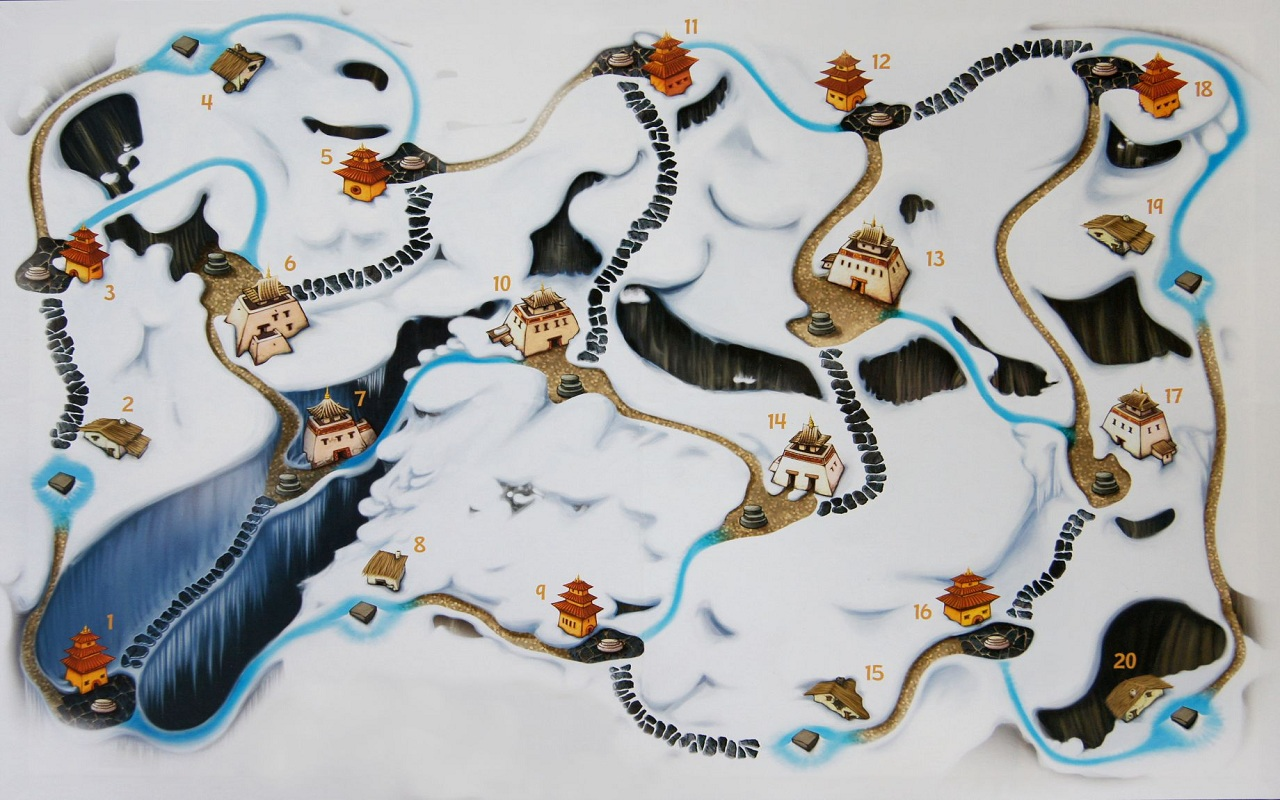
\includegraphics[width=0.7\linewidth]{images/plateau}
	\caption{Plateau du jeu}
	\label{fig:plateau}
\end{figure}

\begin{figure}[h]
	\centering
	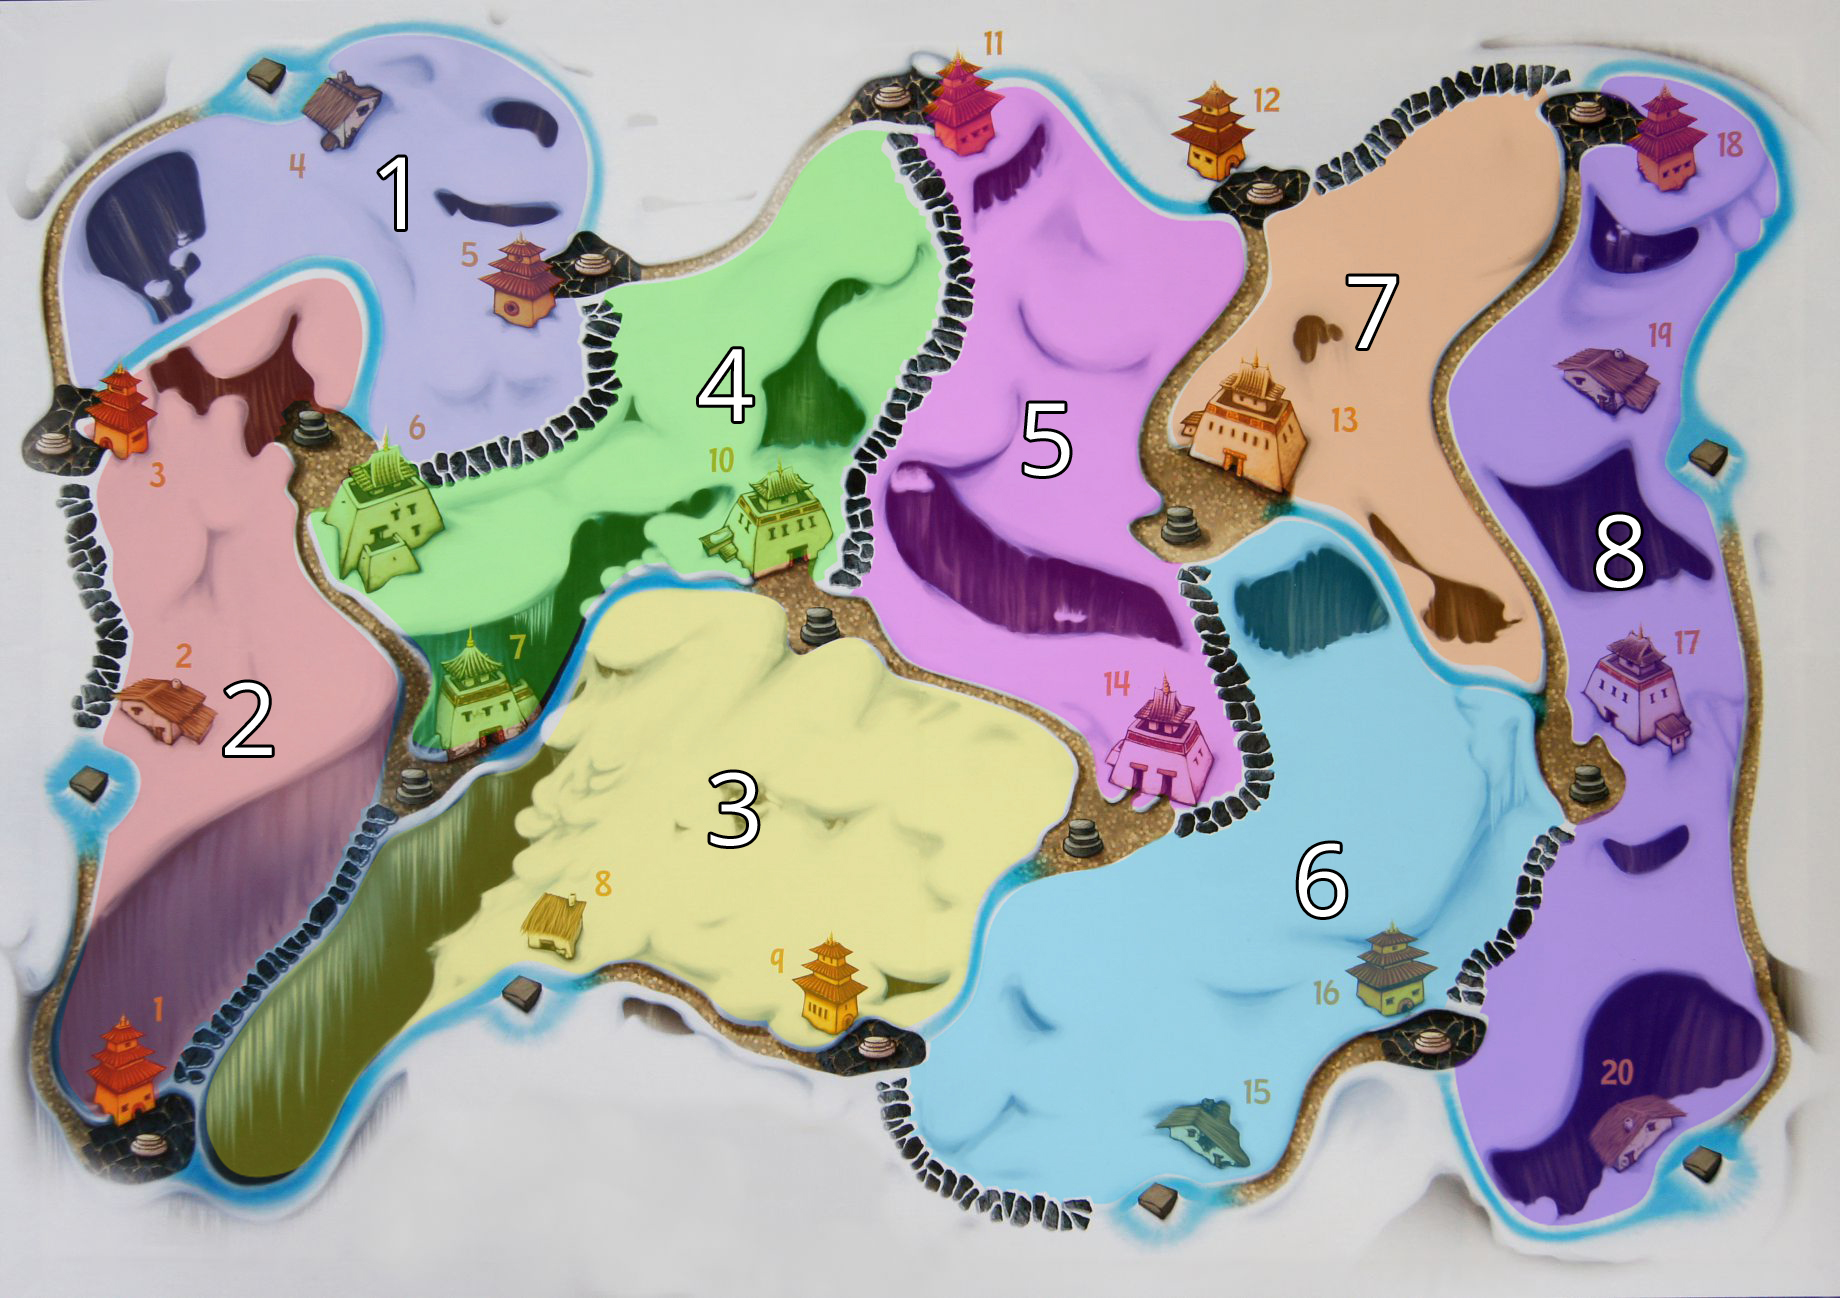
\includegraphics[width=0.7\linewidth]{images/board_regions}
	\caption{Répartitions des régions}
	\label{fig:board_region}
\end{figure}

\begin{figure}[h]
	\centering
	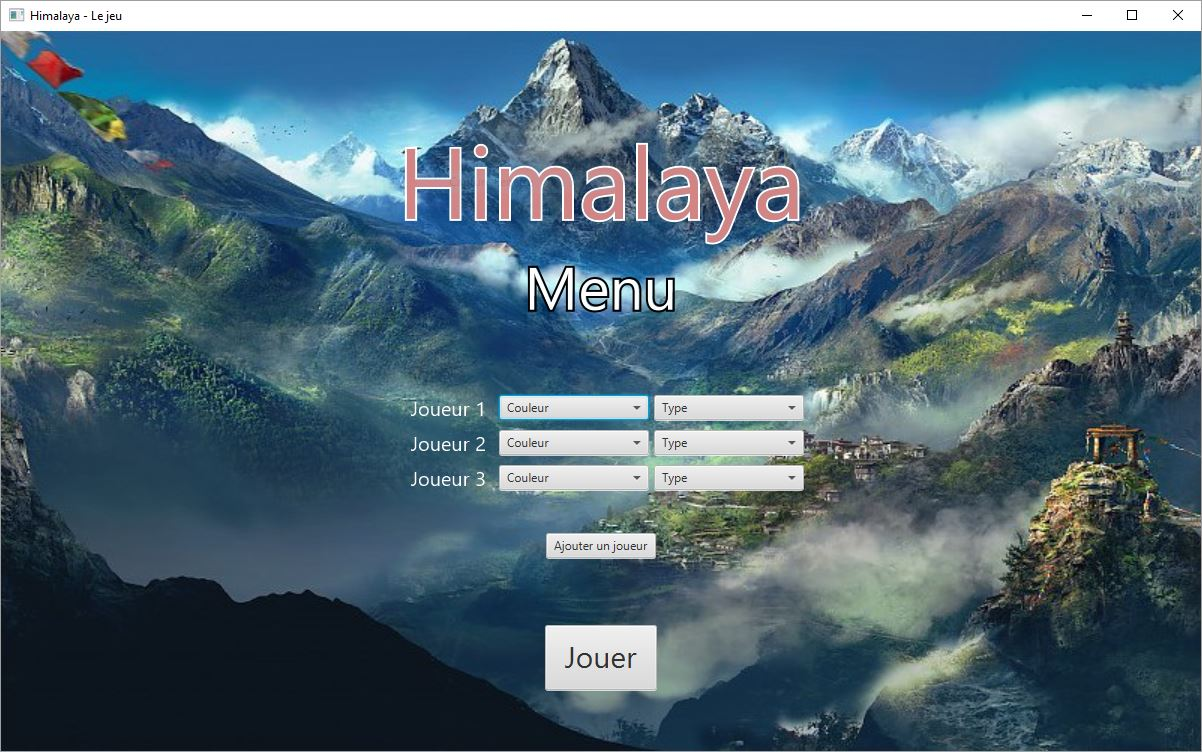
\includegraphics[width=0.9\linewidth]{images/menu}
	\caption{Menu du jeu}
	\label{fig:menu}
\end{figure}

\begin{figure}[h]
	\centering
	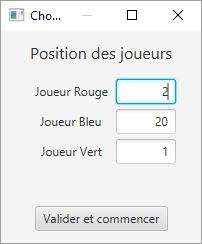
\includegraphics[width=0.4\linewidth]{images/position}
	\caption{Positions initiales}
	\label{fig:pos_init}
\end{figure}

\begin{figure}[h]
	\centering
	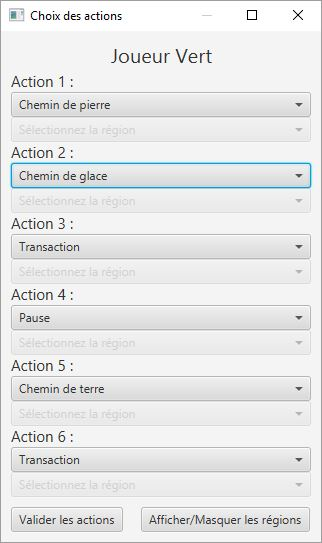
\includegraphics[width=0.4\linewidth]{images/actions}
	\caption{Choix des actions (joueur humain)}
	\label{fig:actions}
\end{figure}

\begin{figure}[h]
	\centering
	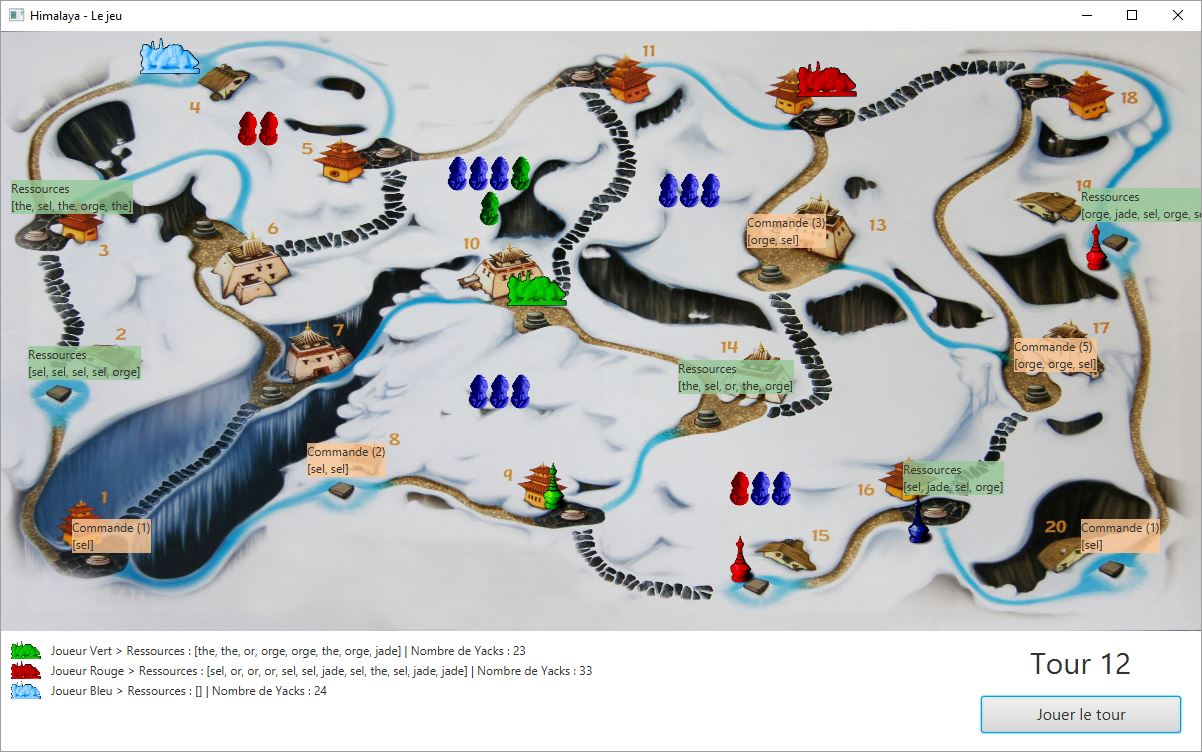
\includegraphics[width=0.9\linewidth]{images/etat_jeu_avance}
	\caption{Déroulement du jeu}
	\label{fig:etat_jeu}
\end{figure}

\begin{figure}[h]
	\centering
	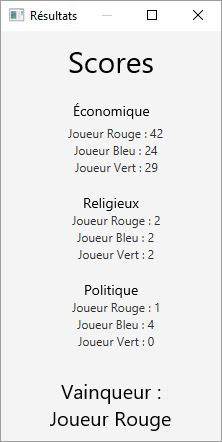
\includegraphics[width=0.3\linewidth]{images/resultats}
	\caption{Résultats de la partie}
	\label{fig:resultats}
\end{figure}

\begin{figure}[h]
	\centering
	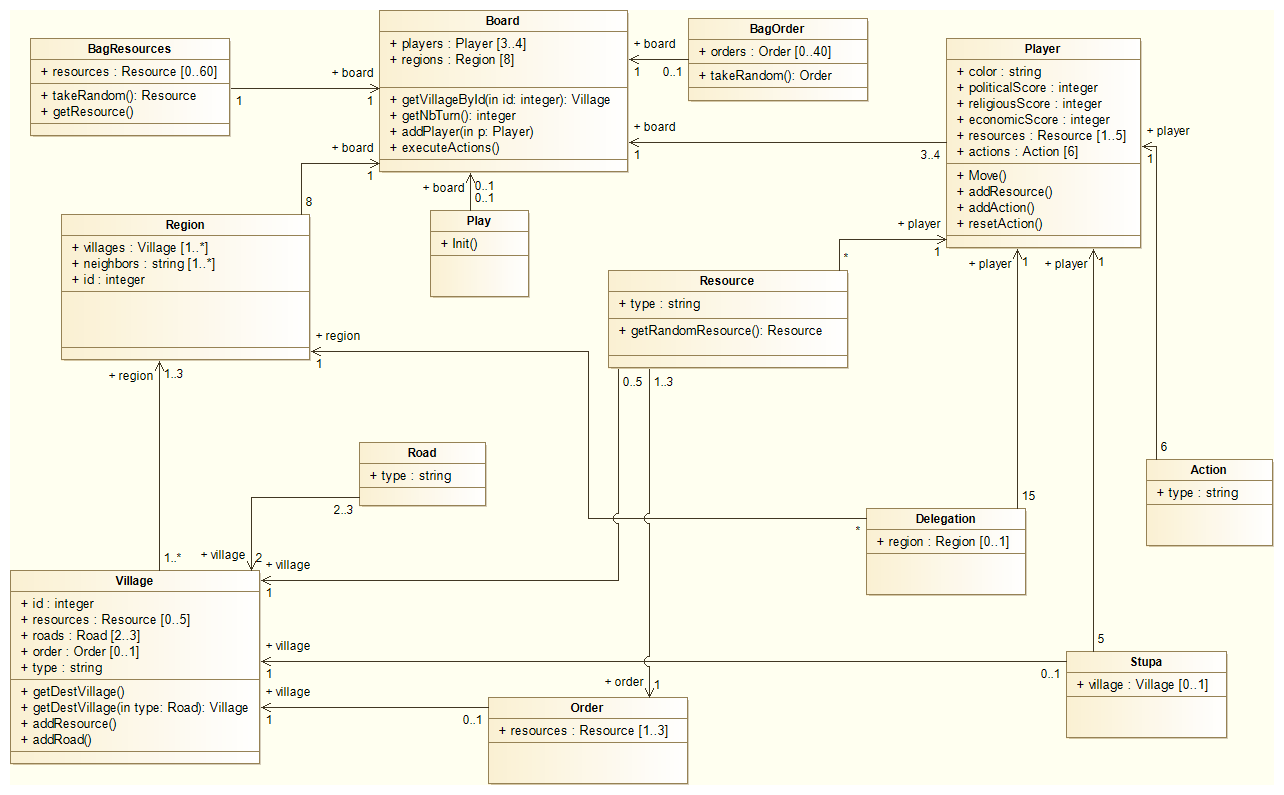
\includegraphics[width=1\linewidth]{images/UML_Himalaya_2}
	\caption{UML Moteur du jeu version 2.5 avant développement}
	\label{fig:UMLCore1}
\end{figure}
\begin{figure}[h]
	\centering
	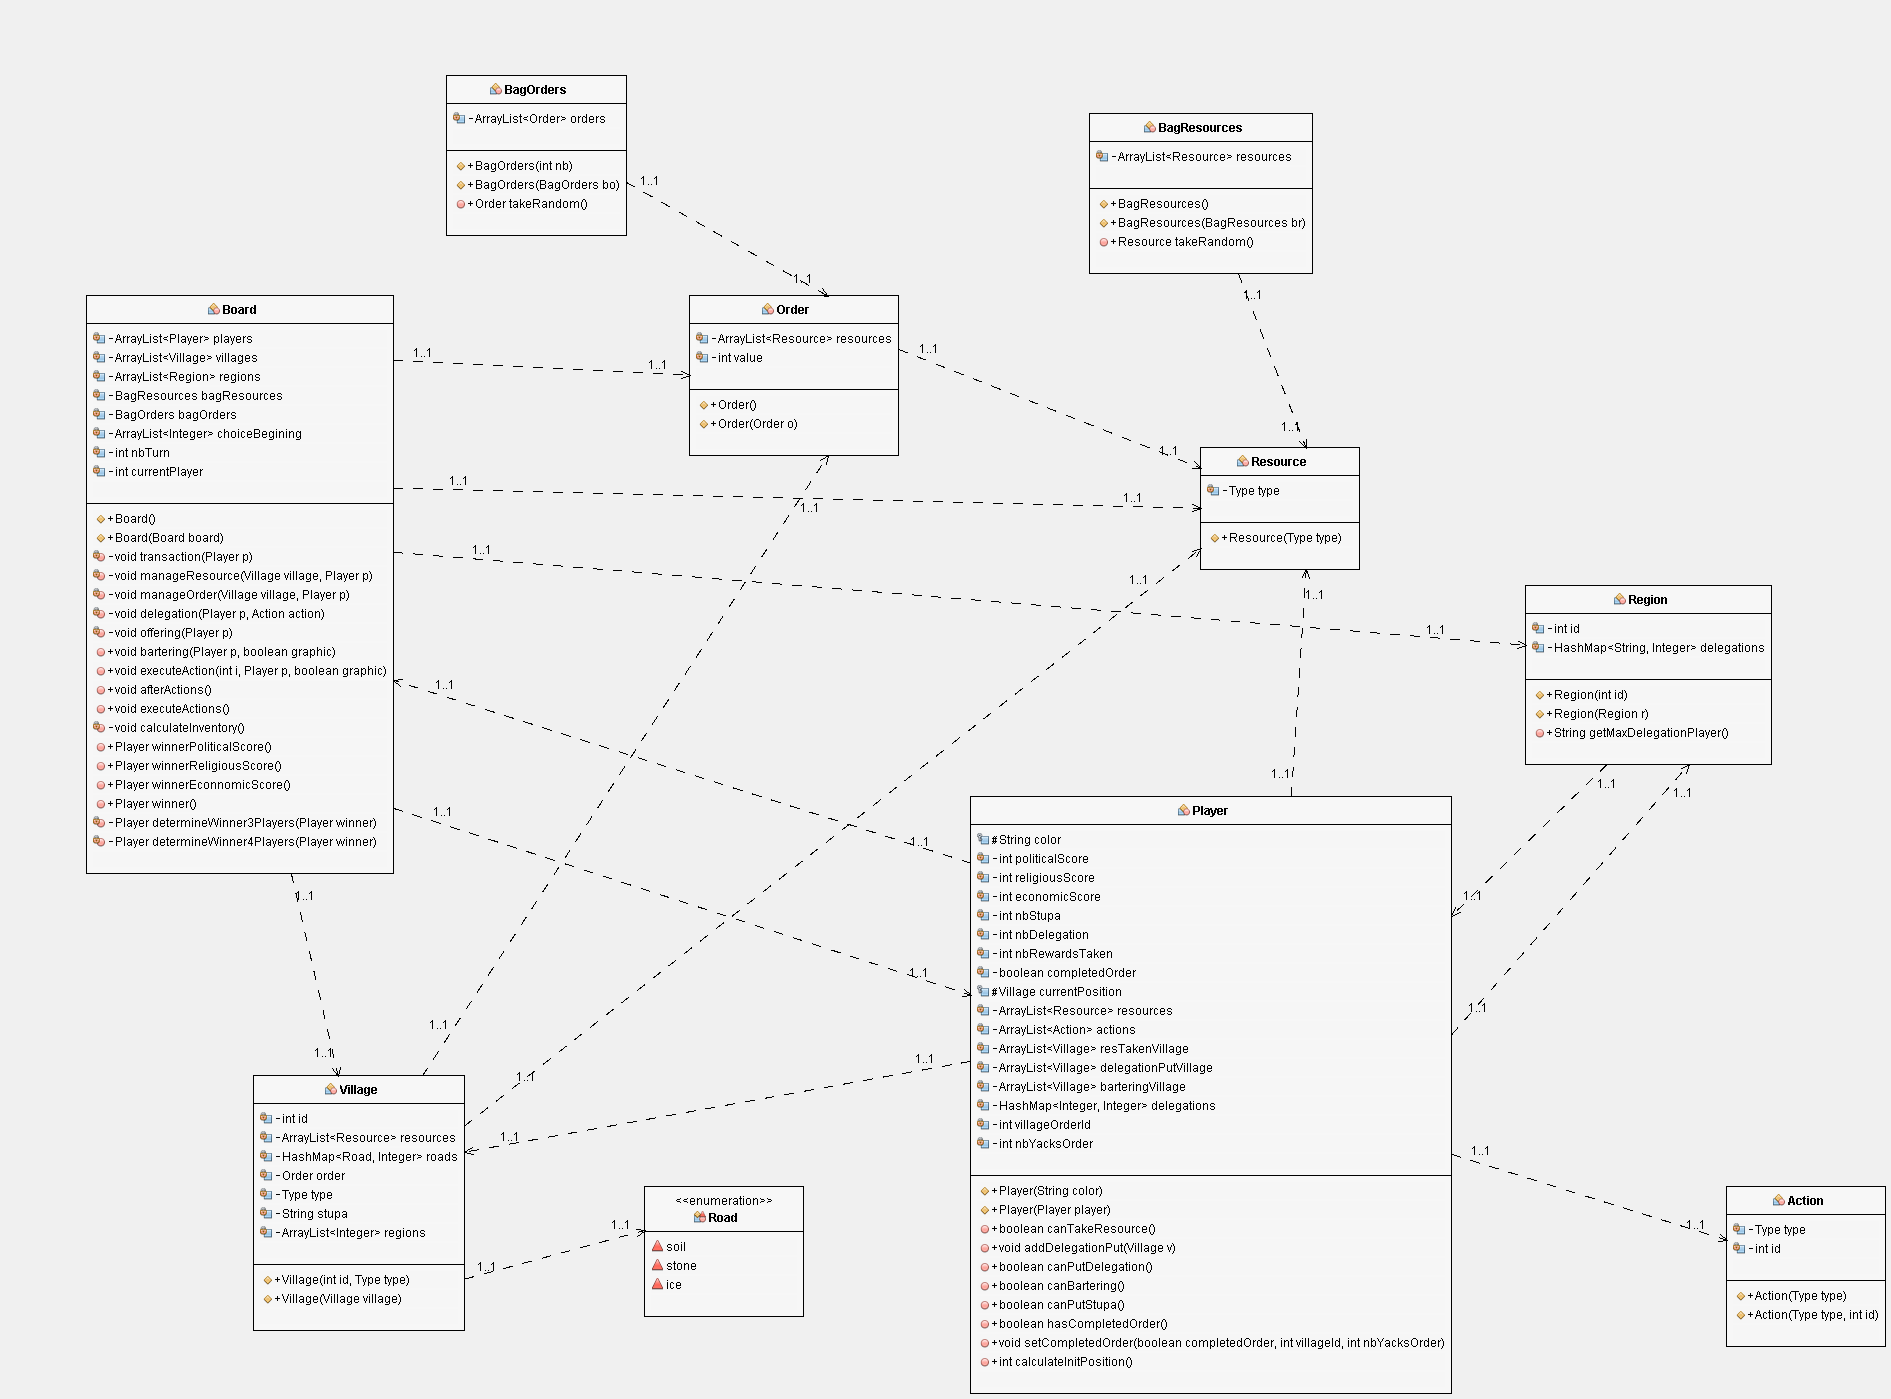
\includegraphics[width=1\linewidth]{images/UML_Himalaya_CORE_3}
	\caption{UML Moteur du jeu version 3.0 après développement}
	\label{fig:UMLCore2}
\end{figure}
\begin{figure}[h]
	\centering
	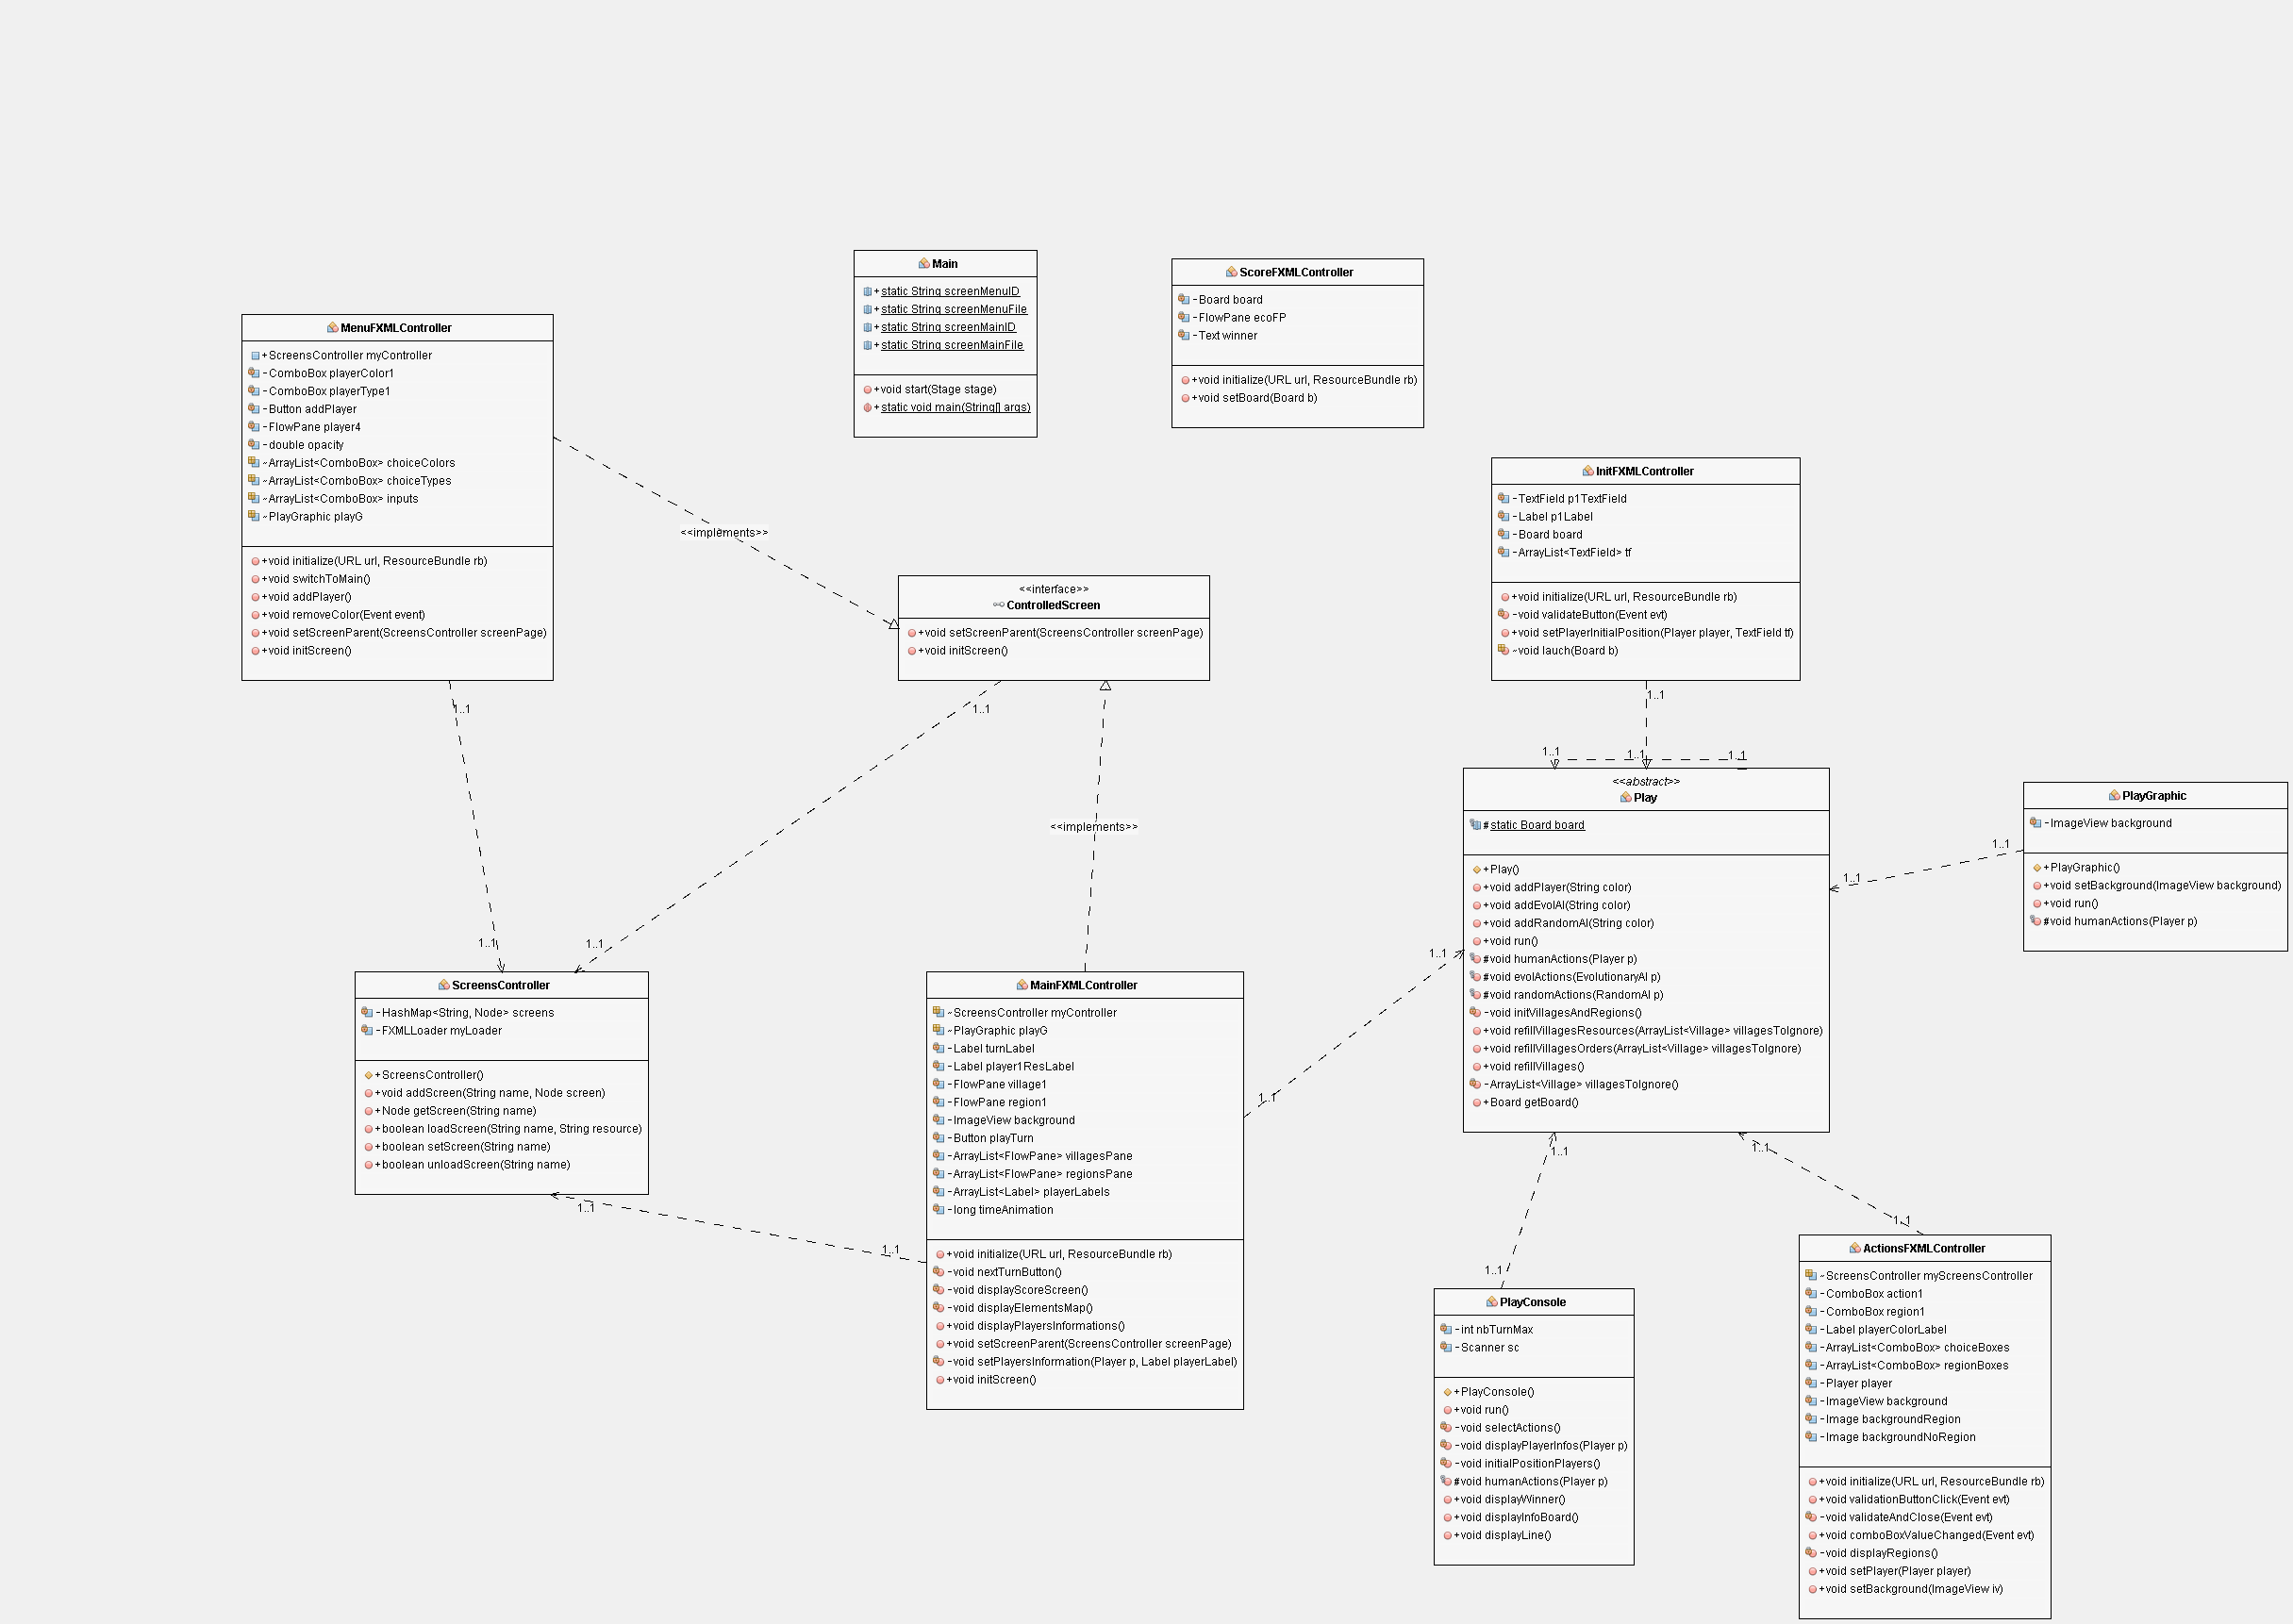
\includegraphics[width=1\linewidth]{images/UML_Himalaya_IHM_1}
	\caption{UML de l'IHM 1.0 après développement}
	\label{fig:UML_IHM}
\end{figure}
\begin{figure}[h]
	\centering
	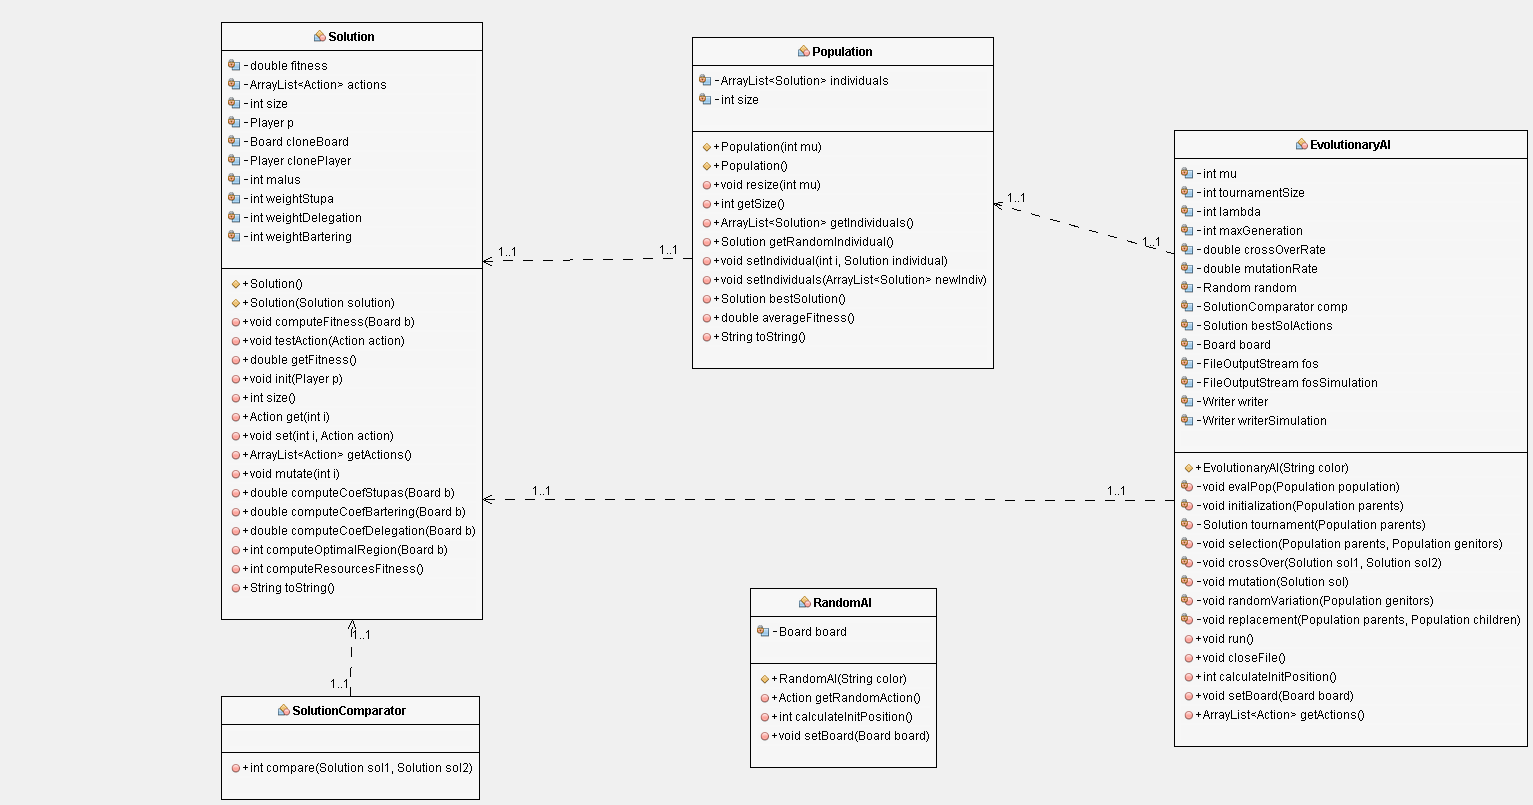
\includegraphics[width=1\linewidth]{images/UML_Himalaya_IA_1}
	\caption{UML de l'IA 1.0 après développement}
	\label{fig:UML_IA}
\end{figure}
